%%%%%%%%%%%%%%%%%%%%%%%%%%%%%%%%%%%%%%%%%%%%%%%%%%%%%%%%%%%%%%%%%%%%%%%%

%%% LaTeX Template for AAMAS-2021 (based on sample-sigconf.tex)
%%% Prepared by Natasha Alechina and Ulle Endriss (version 2020-08-06)

%%%%%%%%%%%%%%%%%%%%%%%%%%%%%%%%%%%%%%%%%%%%%%%%%%%%%%%%%%%%%%%%%%%%%%%%

%%% Start your document with the \documentclass command.
%%% Use the first variant below for the final paper.
%%% Use the second variant below for submission.

% \documentclass[sigconf]{aamas} 
\documentclass[sigconf,anonymous]{aamas} 

%%% Load required packages here (note that many are included already).

\usepackage{balance} % for balancing columns on the final page

\usepackage{listings}
\usepackage{float}
\usepackage{algorithm}
\usepackage{algorithmic}
\usepackage{soul}
\usepackage{amsmath}
\usepackage{wrapfig}
\usepackage{dblfloatfix}
\usepackage{balance}

\setlength{\belowcaptionskip}{-10pt}

%%%%%%%%%%%%%%%%%%%%%%%%%%%%%%%%%%%%%%%%%%%%%%%%%%%%%%%%%%%%%%%%%%%%%%%%

%%% AAMAS-2021 copyright block (do not change!)

\setcopyright{ifaamas}
\acmConference[AAMAS '21]{Proc.\@ of the 20th International Conference on Autonomous Agents and Multiagent Systems (AAMAS 2021)}{May 3--7, 2021}{London, UK}{U.~Endriss, A.~Now\'{e}, F.~Dignum, A.~Lomuscio (eds.)}
\copyrightyear{2021}
\acmYear{2021}
\acmDOI{}
\acmPrice{}
\acmISBN{}

%%%%%%%%%%%%%%%%%%%%%%%%%%%%%%%%%%%%%%%%%%%%%%%%%%%%%%%%%%%%%%%%%%%%%%%%

%%% Use this command to specify your EasyChair submission number.
%%% In anonymous mode, it will be printed on the first page.

\acmSubmissionID{233}

%%% Use this command to specify the title of your paper.

\title[AAMAS-2021 Formatting Instructions]{Auction-based Mechanisms for Resource-elastic Tasks\\in Edge Cloud Computing}

%%% Provide names, affiliations, and email addresses for all authors.

% \author{Paper \#XXX (add number here)}

\author{Mark Towers}
\email{mt5g17@soton.ac.uk}
\affiliation{
    \institution{University of Southampton}
    \city{Southampton}
    \country{United Kingdom}
}
\author{Fidan Mehmeti}
\email{fzm82@psu.edu}
\affiliation{
    \institution{Penn State University}
    \state{Pennsylvania}
    \country{United States}
}
\author{Sebastian Stein}
\email{ss2@ecs.soton.ac.uk}
\affiliation{
    \institution{University of Southampton}
    \city{Southampton}
    \country{United Kingdom}
}
\author{Tom La Porta}
\email{tfl12@psu.edu}
\affiliation{
    \institution{Penn State University}
    \state{Pennsylvania}
    \country{United States}
}
\author{Geeth De Mel}
\email{geeth.demel@uk.ibm.com}
\affiliation{
    \institution{IBM UK}
    \country{United Kingdom}
}
\author{Caroline Rublein}
\email{clr292@psu.edu}
\affiliation{
    \institution{Penn State University}
    \state{Pennsylvania}
    \country{United States}
}

%%% Use this environment to specify a short abstract for your paper.

\begin{abstract}
    Edge Cloud Computing enables computational tasks, such as machine learning models or other AI algoriuthms,
    to be processed at the edge of the network using limited
    computational resources in comparison to larger remote data centres. Because of this, resource allocation and
    management is significantly more important. Existing resource allocation approaches usually assume that tasks
    have inelastic resource requirements (i.e., a fixed amount of bandwidth and computation requirements). However,
    this may result in inefficient resource usage due to unbalanced requirements from tasks that can cause
    bottlenecks. To address this, we propose a novel approach that takes advantage of the elastic nature of resources
    as to time taken for an operation to occur is generally proportional to the allocated resource. This, however,
    makes previous research incompatible with such elasticity. Therefore, we describe this problem formally as an
    optimisation problem and propose a scalable approximation algorithm. To deal with self-interested users, we use a
    technique from multi-agent systems and design to demonstrate a centralised auction mechanism that is incentive
    compatible using the approximation algorithm.
    Moreover, we propose a novel Decentralised Iterative Auction that does not require users to reveal their private
    task value. Using extensive simulations, we show that considering the elasticity of resources leads to a gain in
    utility of around 20\% compared to existing approaches, with the proposed approaches typically achieving 95\% of
    the theoretical optimal.
\end{abstract}

%%% The code below was generated by the tool at http://dl.acm.org/ccs.cfm.
%%% Please replace this example with code appropriate for your own paper.


%%% Use this command to specify a few keywords describing your work.
%%% Keywords should be separated by commas.

\keywords{Edge Cloud Computing; Resource Allocation; Resource-elastic Task; Auctions}

%%%%%%%%%%%%%%%%%%%%%%%%%%%%%%%%%%%%%%%%%%%%%%%%%%%%%%%%%%%%%%%%%%%%%%%%

%%% Include any author-defined commands here.
         
\newcommand{\BibTeX}{\rm B\kern-.05em{\sc i\kern-.025em b}\kern-.08em\TeX}

%%%%%%%%%%%%%%%%%%%%%%%%%%%%%%%%%%%%%%%%%%%%%%%%%%%%%%%%%%%%%%%%%%%%%%%%

\begin{document}

%%% The following commands remove the headers in your paper. For final 
%%% papers, these will be inserted during the pagination process.

\pagestyle{fancy}
\fancyhead{}

%%% The next command prints the information defined in the preamble.

\maketitle 

\section{Introduction}\label{sec:introduction}
In the last few years, cloud computing~\cite{cloud_cite} has become a popular solution for running data-intensive
applications remotely. However, large scale data-centres are not a feasible in application domains that require low
latency or high security and privacy. To deal with such domains, \emph{fog/edge computing} has emerged as a
complementary paradigm allowing tasks to be executed at the edge of networks, close to the user, in small data-centers,
known as \emph{edge clouds}.

As the Internet-of-things grows, fog/edge cloud computing is a key enabling technology in particular for applications
in smart cities, disaster response scenarios, home automation systems, etc. In these applications, low-powered devices
generate data or tasks that can't be processed locally but are impractical to use with standard cloud computing
services. More specifically, in smart cities, these devices could be smart traffic light systems that collect data from
roadside sensors to optimise the traffic light sequence to minimise vehicle waiting times; or to analyse videos feeds
from CCTV cameras of suspicious behaviour. In disaster response, sensor data from autonomous vehicles can be aggregated
to produce real-time maps of devastated areas to help first responders better understand the situation and search for
survivors.

To accomplish these tasks, there are typically several types of resources that are needed, including communication
bandwidth, computational power and data storage resources~\cite{vaji_infocom}, and tasks are generally
delay-sensitive, i.e., have a specific completion deadline. When accomplished, different tasks carry different values
for their owners (e.g., the users of IoT devices or other stakeholders such as the police or traffic authority). This
value will depend on the importance of the task, e.g., analysing current levels of air pollution may be less important
than preventing a large-scale traffic jam at peak times or tracking a criminal on the run. Given that edge clouds are
often highly constrained in their resources~\cite{edge_limitations}, we are interested in allocating tasks to edge
cloud servers to maximize the overall social welfare achieved (i.e., the sum of completed task values). This is
particularly challenging, because users in edge clouds are typically self-interested and may behave
strategically~\cite{Bi2019} or may prefer not to reveal private information about their values to a central allocation
mechanism~\cite{Pai2013}.

An important shortcoming of existing work of resource allocation in edge cloud computing is that it assumes tasks have
strict resource requirements -- that is, each task must be allocate a fixed amount of CPU cycles or bandwidth by a
server. This can cause bottlenecks for certain resources when multiple tasks over-request resources. However, in
practice tasks have flexibility in how resources are allocated given the task is computed within a time limit. This
ability to flexibility allocate resource is additionally important in the case of edge computing due to the limited
resource capacities that servers have in comparison to large data-centre. Using this idea of task resource flexibility,
in this paper, we proposed a new optimisation problem that is incompatible with previous research. Therefore three
mechanisms are proposed for the problem: a greedy mechanism, an incentive compatible centralised auction and a novel
decentralised iterative auction that achieve ~95\% of the theoretical optimal.

%% TODO Make an addition to why this flexibility breaks everything previously
\section{Problem formulation}\label{sec:problem-formulation}
In this section we first describe the system model. Then, we present the optimization problem and prove its NP-hardness.
Final present an example problem to show the affect of the flexible resource allocation compared to fixed resource
allocation.

\begin{figure}[ht]
    \centering
    \includegraphics[width=0.6\linewidth]{fig/system_model.pdf}
    \caption{System Model}
    \label{fig:system_model}
\end{figure}

\subsection{System model}\label{subsec:system-model}
A sketch of the system is shown in Fig.~\ref{fig:system_model}.
We assume that in the system there is a set of servers $I = \{1,2,\ldots,\left|I\right|\}$ servers, which could be edge
clouds that can be accessed either through cellular base stations or WiFi access points (APs). These servers have
different types of limited resources: storage for the code/data needed to run a task (e.g., measured in GB),
computation capacity in terms of CPU cycles per time interval (e.g., measured in FLOP/s), and communication bandwidth
to receive the data and to send back the results of the task after execution (e.g., measured in Mbit/s). We assume
that the servers are heterogeneous in all their characteristics. More formally, we denote the storage capacity of
server $i$ with $S_i$, computation capacity with $W_i$, and the communication (bandwidth) capacity with $R_i$.

There is a set $J = \{1,2,\ldots,\left| J \right|\}$ of different tasks that require service from one of the servers.
\footnote{We focus on a single-shot setting in this paper. In practice, an allocation mechanism would repeat the
allocation decisions described here over regular time intervals, with longer-running tasks re-appearing on consecutive
time intervals. We leave a detailed study of this to future work.} Each task has a value, denoted $v_j$, representing
the value of running the task to its owner. To run any of these tasks on a server requires storing the appropriate
code/data on the same server. This storage size for the task $j$ is denoted as $s_j$ with the rate that the program
is transferred to the server as $s^{'}_j$. For a task to be computed successfully, it must fetch and execute
instructions on a CPU. We consider the total number of CPU cycles required for the program to be $w_j$, where the
number of CPU cycles are assigned to the task per unit of time as $w^{'}_j$. Finally, after the task is run and the
results obtained, the latter need to be sent back to the user. The size of the results for task $j$ is denoted with
$r_j$, and the bandwidth speed it is sent back to the user as $r^{'}_j$. Each task has a deadline, denoted by $d_j$,
as the maximum time for a task to be completed successfully. This time includes: the time required to send the
data/code to the server, run it on the server, and get back the results. We assume that there is an \emph{all} or
\emph{nothing} task execution reward scheme, meaning that the task value is awarded only if entire task loaded,
computed and the results sent back within the deadline.

\subsection{Optimization problem}\label{subsec:optimisation-problem}
Given the aforementioned assumptions from the system model, this requires two allocation mechanisms: the assignment of
tasks to servers and server resources to assigned task. This allocation mechanism is described by the following
optimisation where the variable $x_{i,j} \in \{0, 1\}$ describes if a task $j$ is running on server $i$.

\begin{align}
    \max & \sum_{\forall j \in J} v_j \left(\sum_{\forall i \in I} x_{i,j}\right)\label{eq:objective}\\
    \mbox{s.t.} \nonumber \\
    & \sum_{\forall j \in J} s_j x_{i,j} \leq S_i, &~ \forall i \in I,\label{eq:server_storage_constraint}\\
    & \sum_{\forall j \in J} w^{'}_j x_{i,j} \leq W_i, &~ \forall i \in I,\label{eq:server_computation_constraint}\\
    & \sum_{\forall j \in J} (r^{'}_j + s^{'}_j) \cdot x_{i,j} \leq R_i, &~ \forall i \in I,\label{eq:server_communication_constraint}\\
    & \frac{s_j}{s^{'}_j} + \frac{w_j}{w^{'}_j} + \frac{r_j}{r^{'}_j} \leq d_j, &~ \forall{j \in J},\label{eq:task_deadline}\\
    & 0 < s^{'}_j < \infty, &~ \forall{j \in J,}\label{eq:loading_speeds}\\
    & 0 < w^{'}_j < \infty, &~ \forall{j \in J,}\label{eq:compute_speeds}\\
    & 0 < r^{'}_j < \infty, &~ \forall{j \in J,}\label{eq:sending_speeds}\\
    & \sum_{\forall i \in I} x_{i,j} \leq 1, &~ \forall j \in J,\label{eq:server_task_allocation}\\
    & x_{i,j} \in \{0, 1\}, &~ \forall{i \in I},\forall{j \in J}.\label{eq:task_allocation}
\end{align}

The objective (Eq.\eqref{eq:objective}) is to maximize the total value over all tasks (i.e., the social welfare) that
are completed within the deadline (Eq.~\eqref{eq:task_deadline}. Constraints~\eqref{eq:server_storage_constraint},
~\eqref{eq:server_computation_constraint} and~\eqref{eq:server_communication_constraint} related to the finite resource
capacity of the servers, storage, computation and communication (bandwidth) respectively.
Constraint~\eqref{eq:server_storage_constraint} relates to the finite storage capacity for the task to store code/data
used to compute. With Eq.\eqref{eq:server_computation_constraint} being the finite computation capacity of each server.
The communication constraint (Eq.~\eqref{eq:server_communication_constraint}) comprises of two parts: the first for the
loading of the data/code onto the server, and the second for sending back the results to the user.
Constraint~\eqref{eq:task_deadline} forces the task to be completed within the task deadline, that being the sum of
time taken for all of the stages to complete in series (i.e.. loaded task onto server, computing the task, sending the
results back to the user). Note that if a task is not run on any server, this constraint can be satisfied by choosing
arbitrarily high bandwidth and CPU rates (as these resources do not use up any servers' resources in
Eq.~\eqref{eq:server_storage_constraint},~\eqref{eq:server_computation_constraint}
and~\eqref{eq:server_communication_constraint} when not allocated to server). The rates for each stage
($s^{'}_j$, $w^{'}_j$ and $r^{'}_j$) are all positive and finite (Eqs.~\eqref{eq:loading_speeds}
,~\eqref{eq:compute_speeds},~\eqref{eq:sending_speeds}). Further, every task is served by at most one server
(Eq.\eqref{eq:server_task_allocation}) as each task is either served or not by each server
(Eq.\eqref{eq:task_allocation}). \\


Using this optimisation problem, this is an extension of the knapsack problem that is well-studied and known to be
NP-hard with pseudo-polynomial time complexity using dynamic programming.
\begin{theorem}
    The optimisation problem as described in section~\ref{subsec:optimisation-problem} is NP-hard.
\end{theorem}
\begin{proof}
    The optimization problem without the constraint~\eqref{eq:task_deadline} is a 0--1 multidimensional knapsack
    problem~\cite{knapsackproblems_2004}, which is a generalization of a simple 0--1 knapsack problem. The latter is an
    NP-hard problem~\cite{knapsackproblems_2004}. Given this, it follows that the 0--1 multidimensional knapsack problem
    is also NP-hard. Since optimization problem (Eqs~\eqref{eq:objective} -~\eqref{eq:task_allocation}) is a
    generalization of a 0--1 multidimensional knapsack problem, it follows that it is NP-hard as well.
\end{proof}

\subsection{Example Problem Case}\label{subsec:example-problem-case}
Before we propose our novel allocation mechanisms for the allocation problem with elastic resources, we briefly
outline an example to illustrates why considering this elasticity is important. In this example, there are 12 potential
tasks and 3 servers (the exact settings can be found in table~\ref{table:example_tasks_properties} for the tasks and
table~\ref{table:example_servers_properties} for the servers). The figures~\ref{fig:fixed_resources_speeds}
and~\ref{fig:flexible_resources_speeds} represents each server as a group of three bars, each relating to the each
server's resource types, with the percentage of resources used by a task being the size of the bar.

\begin{figure}[th]
    \centering
    \includegraphics[width=\linewidth]{fig/allocation/fixed_optimal_allocation.pdf}
    \caption{Optimal solution with fixed resource speeds}
    \label{fig:fixed_resources_speeds}
\end{figure}

Figure~\ref{fig:fixed_resources_speeds} shows the best possible allocation if tasks have fixed resource speeds (that
were set by minimising the total amount of resources to be completed within the deadline). Here, only 9 of the tasks
are run, resulting in a total social welfare of 980 due to server 1 and 2's limited computational capacity and server
3' limited communication capacity.

\begin{figure}[th]
    \centering
    \includegraphics[width=\linewidth]{fig/allocation/flexible_optimal_allocation.pdf}
    \caption{Optimal solution with elastic resources. Compared to the fixed allocation, the elastic allocation is able
    to fully use all of its resources}
    \label{fig:flexible_resources_speeds}
\end{figure}

In contrast to figure~\ref{fig:fixed_resources_speeds}, Figure~\ref{fig:flexible_resources_speeds} depicts the optimal
allocation if elastic resources are considered. Here, all of the resources are used by the servers whereas the fixed
example~\ref{fig:fixed_resources_speeds} cant do this. In total, the elastic approach manages to schedule all 12 tasks
within the resource constraints, achieving a total social welfare of 1200 (an 18\% improvement over the fixed approach).

\begin{table}[h]
    \begin{tabular}{|c||c|c|c|}
        \hline
        Name & $S_i$ & $W_i$ & $R_i$ \\ [0.5ex] \hline\hline
        Server 1 & 400 & 100 & 220 \\ \hline
        Server 2 & 450 & 100 & 210 \\ \hline
        Server 3 & 375 & 90 & 250 \\ \hline
    \end{tabular}
    \caption{Table of server attributes}
    \label{table:example_servers_properties}
\end{table}

\begin{table}[h]
    \begin{tabular}{|c||c|c|c|c|c||c|c|c|}
        \hline
        Name & $v_j$ & $s_j$ & $w_j$ & $r_j$ & $d_j$ &  $s^{'}_j$ & $w^{'}_j$ & $r^{'}_j$ \\ [0.5ex] \hline\hline
        Task 1 & 100 & 100 & 100 & 50 & 10 & 30 & 27 & 17 \\ \hline
        Task 2 & 90 & 75 & 125 & 40 & 10 & 22 & 32 & 15 \\ \hline
        Task 3 & 110 & 125 & 110 & 45 & 10 & 34 & 30 & 17 \\ \hline
        Task 4 & 75 & 100 & 75 & 35 & 10 & 27 & 21 & 13 \\ \hline
        Task 5 & 125 & 85 & 90 & 55 & 10 & 24 & 28 & 17 \\ \hline
        Task 6 & 100 & 75 & 120 & 40 & 10 & 20 & 32 & 16 \\ \hline
        Task 7 & 80 & 125 & 100 & 50 & 10 & 31 & 30 & 19 \\ \hline
        Task 8 & 110 & 115 & 75 & 55 & 10 & 30 & 22 & 20 \\ \hline
        Task 9 & 120 & 100 & 110 & 60 & 10 & 27 & 29 & 24 \\ \hline
        Task 10 & 90 & 90 & 120 & 40 & 10 & 25 & 30 & 17 \\ \hline
        Task 11 & 100 & 110 & 90 & 45 & 10 & 30 & 26 & 16 \\ \hline
        Task 12 & 100 & 100 & 80 & 55 & 10 & 24 & 24 & 22 \\ \hline
    \end{tabular}
    \caption{Table of task attributes. The columns ($s^{'}_j$, $w^{'}_j$, $r^{'}_j$) are fixed speeds which are not
    considered by the flexible resource allocation.}
    \label{table:example_tasks_properties}
\end{table}
\section{Flexible resource allocation mechanisms}
\label{sec:flexible-resource-allocation-mechanisms}
As explained earlier, previous research outlined in Section~\ref{sec:introduction} does not consider resource-elastic tasks. Therefore, in this section, we propose three mechanisms for solving our optimisation problem: an approximation algorithm and two auction-based mechanisms. As the greedy algorithm is a centralised approximation algorithm it has several shortcomings: it assumes that users reveal private task information truthfully, and it assumes there is a central point of control for all server allocation decisions. We address each of these shortcomings in the subsequent two auction mechanisms. 

\subsection{Greedy algorithm}
\label{subsec:greedy-algorithm}
To solve knapsack problems, a greedy approximation algorithm is often used~\cite{sahni1975approximate}. Therefore, we have applied a similar approach to our problem. However, due to the elastic nature of task resources, a novel additional stage is required. More specifically, the greedy algorithm (pseudo code can be found in Section 2 of the supplementary material) has two stages: the first stage sorts the tasks based on a task priority function. The novel second stage uses the sorted tasks to apply two heuristics; the first for selecting a server based on available server resources and the second to allocate resources based on the available server resources and the required resources of the task. %% TODO Add an explanation about the heuristics

\subsubsection{Lower bound of the greedy algorithm}
\label{subsubsec:greedy-lower-bound}
%% TODO look at again
Due to the server selection and resource allocation heuristics not taking into account other tasks, the lower bound of the greedy algorithm is $\frac{1}{OPT}$ (where $OPT$ is the optimal social welfare) where the task value is used for the task priority function. However in testing, we found that the task value is not the best task priority heuristic as it does not consider the effect of deadlines or the required resources of the task. This is due to not considering other tasks resource requirements when allocating resources, no matter of the server selection or resource allocation functions, the algorithm cannot guarantee that any subsequent tasks could be allocated to any server after the first task is allocated. As a result, the algorithm can be guaranteed to achieve at least $\frac{1}{OPT}$ of the optimal social welfare by sorting the tasks by task value ($v(j) = j_v$).

\subsubsection{Computational complexity of greedy algorithm}
\label{subsubsec:greedy-time-complexity}
The computational complexity of the greedy algorithm is $O(\left|J\right| \left|I\right| + n^3)$, where $\left|J\right|$ is the number of tasks, $\left|I\right|$ is the number of servers and $n$ is the discretization of the server and task resources. This assumes that all of the heuristics take constant complexity for their evaluation. Therefore, for the first stage of the algorithm where the tasks are sorted the complexity is $O(\left|J\right| \log(\left|J\right|))$. While for the second stage, for each task the server selection heuristic is applied to each server, which has a complexity of $O(\left|J\right| \left|I\right|)$. Then for resource allocation, to get the best allocation requires checking if all of the server resources depends on the server discretization.\footnote{Faster solutions exist for finding the best allocations like branch and bound or Karush–Kuhn–Tucker conditions.} Therefore, the overall complexity is $O(\left|J\right| \log(\left|J\right|) + \left|J\right| \left|I\right| + n^3) = O(\left|J\right| \left|I\right| + n^3)$.

\subsection{Critical value auction}
\label{subsec:critical-value-auction}
A potential shortcoming of the greedy algorithm is that it assumes truthful reporting of the task characteristics, including its value. In realistic settings with self-interested task owners, if the greedy algorithm was used to allocate resources such that the value is the price paid, the system would be open to manipulation and the misreporting of task attributes. Therefore, in this section we propose the Critical Value auction, a strategyproof (weakly dominant incentive compatible) auction that means users have no incentive to misreport task attributes.

The auction is based on Single Parameter Auctions~\cite{nisan2007algorithmic} (Section~9.5.4), where the price for a task is the minimum value revealed by a task such that it would still be allocated to any server, called the \emph{critical value}. The auction (pseudo code can be found in Section 3 of the supplementary material) is implemented using the greedy algorithm, from Subsection~\ref{subsec:greedy-algorithm}, for finding both the initial allocation of tasks and critical value for each task (in a modified form). Because of this, the auction inherits the social welfare properties of the greedy algorithm using the same modular functions.

The auction works by first finding the initial allocation of tasks based on task's revealed values using the greedy algorithm. Then for each allocated task its critical value is determined that is equal to the minimum value the task could report such that it would still be allocated. This is done by modifying the greedy algorithm such that after every task is allocated to a server, a check is done to see if the critical value task could be allocated to any server.\footnote{This check has linear time complexity as it assumes that a server would allocate all of its available resources to the critical task. However, for the bandwidth resources, this must be split between loading and sending resources to check if the deadline can be met.} Once the critical value task cannot be allocated to any server, then the task priority of the previously allocated task must be equal to the critical value task's minimum task priority.\footnote{We assume that the critical task would be placed above the task if the task priorities are equal. To avoid this, the owner can add a small amount of the value to increase the task priority, placing the critical task ahead.} The critical value is found by taking the inverse of the task priority function with critical task's attributes and task priority of the previous task.

\subsubsection{Computational complexity of critical value auction}
\label{subsubsec:critical-value-auction-time-complexity}
Using the argument from Subsection~\ref{subsubsec:greedy-time-complexity}, the computational complexity of the greedy algorithm is $O(\left|J\right| \left|I\right|)$. The computational complexity of the auction is $O(\left|J\right|^2 \left|I\right|)$, as the auction repeats the greedy algorithm  $\left|J\right|$ times. For the first stage of the auction, the greedy algorithm finds the initial allocation, with the second stage finding the critical value of each allocated task. For the second stage, it uses a modified version of the greedy algorithm, which has a computational complexity of  $O(\left|J\right| \left|I\right|)$. After each task is allocated, a check runs to see if the critical task can be allocated to any server. This check has linear time complexity, as the server's bandwidth resources must be split between task loading and sending speeds. The second modification calculates a task's critical value that takes constant time. Therefore, the computational complexity is due to running  the greedy algorithm ($O(\left|J\right| \left|I\right|)$) plus the complexity of checking after each task for each server ($O(\left|J\right| \left|I\right|)$). Therefore the computational complexity for calculating the critical value of an individual task is $O(\left|J\right| \left|I\right|)$. Thus, combining the two, the overall time complexity is $O(\left|J\right|^2 \left|I\right|)$, as the critical value needs to be calculated for every task.

\subsubsection{Critical value auction strategyproof requirement}
\label{subsubsec:critical-value-auction-strategyproof}
Previous work~\cite{nisan2007algorithmic} (in particular Lemma~11.9) has proven that if the allocation decision is monotonic and critical value payments are used, then the auction is strategyproof (weakly dominant incentive compatible). In our setting, a monotonic allocation means that if an agent is allocated for a given set of parameters, say $\theta_j = (v_j, s_j, w_j, r_j, d_j)$, it would remain allocated when  reporting $\theta'_j = (v'_j, s'_j, w'_j, r'_j, d'_j) $, with $v'_j \geq v_j$, $s'_j \leq s_j$, $w'_j \leq w_j$, $r'_j \leq r_j$, and $d'_j \geq d_j$. This condition can be achieved by using a task priority function that enforces this monotonicity relationship. Specifically, reporting $\theta'_j$ must result in a task priority at least as high as reporting $\theta_j$. In this case, the agent would be evaluated earlier in the greedy order and if $\theta_j$ was allocated, $\theta'_j$ would also remain allocated. Here, it is important to enforce that agents are never allocated more than their requested $s_j$, $w_j$ and $r_j$, and that results are returned exactly on the deadline $d_j$, to ensure that truthful reporting of these parameters is incentivised (as agents maximise the task priority function in this way). This can be easily achieved by post-processing a given solution. One example family of task priority functions that meets the required monotonicity requirement is $\frac{\alpha(v_j, d_j)}{\beta(s_j, w_j, r_j)}$, where  $\alpha$ and $\beta$ are monotonically increasing in their parameters. In our experiments, we use $\frac{v_j \cdot d_j}{s_j + w_j + r_j}$.

\subsection{Decentralised iterative auction}
\label{subsec:decentralised-iterative-auction}
In some applications of edge computing, keeping the value of a task secret is important, especially if the infrastructure is shared by multiple companies or by partners of a military coalition. Therefore, we propose a novel decentralised iterative auction. In this auction, servers offer to complete tasks for a given price, which is equal to the sum of prices (i.e., the server's revenue) of other tasks that the task would displace, plus a bid increment. Task owners either reject or accept these prices, potentially displacing other tasks, and the process continues iteratively until the allocation converges.

%based on the pricing principle of the VCG auction~\cite{vickrey,Clarke,groves}. In the VCG auction, the price of an item is the difference in social welfare for when the item is sold and when it is not. Our proposed novel auction uses this VCG mechanism except using revenue instead of social welfare to calculate a price. This allows tasks to not need to reveal their task value to the servers as the task price (and not task value) is used to update task prices. 

\begin{algorithm}
    \caption{Decentralised iterative auction}
    \label{alg:decentralised-iterative-auction}
    \begin{algorithmic}
        \REQUIRE $J'$ is the set of unallocated tasks, initially the set of tasks
        \REQUIRE $I$ is the set of servers
        \REQUIRE $P(i, j)$ is the solution to the server revenue optimisation problem in Subsection~\ref{subsubsec:decentralised-iterative-problem} using the server $i$ and new task $j$. 
        \REQUIRE $\leftarrow_R A$ randomly select an element from set $A$
        
        \WHILE{$|J'| > 0$}
            \STATE{$j \leftarrow_R J'$}
            \STATE{$\min_p \leftarrow \infty$}
            \STATE{$\min_i \leftarrow \text{NULL}$}
            \FORALL{$i \in I$}
                \STATE{$p \leftarrow \max(R_i - P(i, j) + b_i, r_i)$}
                \IF{$p < \min_p$}
                    \STATE{$\min_p \leftarrow p$}
                    \STATE{$\min_i \leftarrow i$}
                \ENDIF
            \ENDFOR
            \IF{$\min_p \leq v_j$}
                \STATE{$p_j \leftarrow \min_p$}
                \STATE{$J_{\min_i} \leftarrow J_{\min_i} \cup \{j\}$}
                \STATE{Add deallocated tasks from server $\min_i$ to $J'$}
            \ENDIF
            \STATE{$J' \leftarrow J' \setminus \{j\}$}
        \ENDWHILE
    \end{algorithmic}
\end{algorithm}

Formally, tasks have a price, $p_j$, initially set to 0, while each server $i$ has four additional variables: $R_i$ for revenue, $b_i$ for bid increment, $r_i$ for reserve price and $J_i$ for the set of currently allocated task. 

The pseudo code for the auction is  shown in Algorithm~\ref{alg:decentralised-iterative-auction}. For simplicity, we show this as a sequential algorithm, but the respective owners of each task $j$ could be executing this in parallel and in a decentralised manner. In more detail, the auction  works by tasks individually advertising all of their attributes except their value to all of the servers, who each reply with a price to run. This price is the difference between the current server revenue and the revenue when the task is allocated with a price of zero (solved with the optimisation problem in Subsection~\ref{subsubsec:decentralised-iterative-problem}), plus a bid increment. This increment is added to ensure that the server revenue increases by accepting the task. A reserve price can also be implemented by the servers to help increase revenue or reduce the number of rounds required until task prices converge. Once all of the servers have returned a price to the task, the task can compare the prices with its private value. Our algorithm (Algorithm~\ref{alg:decentralised-iterative-auction}) assumes the tasks will choose the minimum price by a server (although other strategies are possible). On selecting a server, in order for the task to be allocated, the server may displace other tasks who must re-advertise their task attributes. The auction stops when all of the tasks have either been allocated to a server or cannot be allocated to any server due to the minimum price of any server being greater than the task's value. Section~\ref{sec:empirical-results} investigates the impact of different bid increments and reserve prices on the system's social welfare, revenue and rounds required for prices to converge. 

\subsubsection{Server revenue optimisation problem}
\label{subsubsec:decentralised-iterative-problem}
To find the price for a new task $j'$, the server $i$ calculates the optimal revenue if the task was allocated with a price of 0. This has a similar formulation to the optimisation problem in Section~\ref{sec:problem-formulation}, except that it is for a single server. The additional variables used are $p_j$ for the price of task $j$, and $x_j$ that denotes whether task $j$ is allocated to the server or not.

\begin{align}
    \max & \sum_{\forall j \in J_i} p_j x_j\label{eq:dia-objective}\\
    \mbox{s.t.} \nonumber \\
    & \sum_{\forall j \in J_i} s_j x_j + s_{j'} \leq S_i,\label{eq:dia-server-storage-constraint}\\
    & \sum_{\forall j \in J_i} w'_j x_j + w_{j'} \leq W_i, \label{eq:dia-server-computation-constraint}\\
    & \sum_{\forall j \in J_i} (r'_j + s'_j) \cdot x_j + (r'_{j'} + s'_{j'}) \leq R_i, \label{eq:dia-server-communication-constraint}\\
    & \frac{s_j}{s'_j} + \frac{w_j}{w'_j} + \frac{r_j}{r'_j} \leq d_j, &~ \forall j \in J_i \cup \{j'\}, \label{eq:dia-task-deadline}\\
    & x_j \in \{0,1\}, &~ \forall{j \in J_i}. \label{eq:dia-task-allocation}
\end{align}

The objective (Eq.~\eqref{eq:dia-objective}) maximises the server revenue (i.e. the price of all completed tasks which does not include the new task $j'$, whose price is zero). The server resource capacity constraints (Eqs.~\eqref{eq:dia-server-storage-constraint},~\eqref{eq:dia-server-computation-constraint} and~\eqref{eq:dia-server-communication-constraint}) are similar to the constraints in the standard model set out in Subsection~\ref{subsec:optimisation-problem} except for the assumption that the new task $j'$ is running. The deadline constraint (Eq.~\eqref{eq:dia-task-deadline}) is identical to the standard formulation constraint. 

\subsubsection{Decentralised iterative auction properties}
\label{subsubsec:decentralised-iterative-auction-properties}
For our proposed auction, we consider strategyproofness and economic efficiency. Despite the decentralised nature of the auction and the fact that users do not reveal a task's value, they are still potentially able to profit from misreporting task attributes. One example would be to misreport a task's attributes to allow another task to make decisions that would otherwise result in the misreporting task from being deallocated from a server. Therefore, the auction is not strategyproof. However, in Subsection~\ref{subsec:dia-misreport-task-attributes}, we show that through extensive search, it is extremely difficult to profit from misreporting.

Due to the allocation of tasks to servers being random until servers become full, the initial allocation and the random selection of tasks can result in the system getting stuck in local system revenue maxima rather than the global maximum. As a result, the auction is not economically efficient, as in some cases the system could be improved. However,  Subsection~\ref{subsec:evaluation-of-the-auction-mechanisms} shows that the auction typically gets within 95\% of the optimal social welfare.

%% This must be placed here such that it appears at the bottom of the page
\begin{figure*}[bp]
    \centering
    \includegraphics[width=\textwidth]{figs/greedy/social_welfare.pdf}
    \caption{Social welfare of the server relaxed optimal, flexible resource allocation, greedy algorithm and fixed resource allocation for a range of model settings.}
    \label{fig:greedy-algorithm-comparison}
\end{figure*}

\subsection{Properties of the proposed algorithms}
In this section, we have presented three mechanisms to solve the optimisation problem proposed in Subsection~\ref{subsec:optimisation-problem}. Table~\ref{tab:algorithms-properties} considers a range of important properties that allow an easy comparison between the proposed algorithms.

\label{subsec:proposed-algorithms-properties}
\begin{table}[H]
    \caption{Properties of the proposed algorithms: greedy algorithm, critical value auction and the
             decentralised iterative auction}
    \label{tab:algorithms-properties}
    \begin{tabular}{|p{2.25cm}|p{1.5cm}|p{1.25cm}|p{2cm}|}
        \hline
        \textbf{Properties} & Greedy algorithm & Critical value auction & Decentralised iterative auction \\ \hline
        Strategyproofness & No & Yes & No \\ \hline
        Optimality & No  & No & No \\ \hline
        Scalability & Yes & Yes & No \\ \hline
        Task information & All & All & All except the task value \\ \hline
        Decentralisation & No  & No  & Yes \\ \hline
    \end{tabular}
\end{table}
\section{Empirical Evaluation}\label{sec:empirical-evaluation}
To test the algorithms presented in section~\ref{sec:flexible-resource-allocation-mechanisms}, synthetic models have
been used to generate a list of tasks and servers. These models have been handcrafted with each attribute being
generated from a Gaussian distribution with a mean and standard deviation.

To compare the greedy algorithm to the optimal elastic allocation, a branch and bound was implemented to solve the
optimisation problem in section~\ref{subsec:optimisation-problem}. In order to compare to fixed speed equivalent models,
the minimum total resource required to run the job is found and set as the resource speeds for all of the tasks, with
the optimal solution for running the job with the fixed speeds is found as well. To implement the greedy mechanism, the
value density function was $\frac{v_j}{s_j + w_j + r_j}$, server selection was
$\text{argmin}_{\forall i \in I} S^{'}_i + W^{'}_i + R^{'}_i$ and the resource allocation was
$\text{min} s^{'}_j + w^{'}_j + r^{'}_j$ for job $j$ and servers $I$.

% Greedy mechanisms
\begin{figure}[h]
    \centering
    \includegraphics[width=\linewidth]{figs/empirical_evidence/greedy_mechanism}
    \caption{Comparison of the social welfare for the greedy mechanism, optimal, relaxed problem, time limited branch and bound}
    \label{fig:greedy_mechanism_comparison}
\end{figure}
As figure~\ref{fig:greedy_mechanism_comparison} shows, the greedy mechanism achieves 98\% of the optimal solution for
the small models, the mechanism achieves within 95\% for larger models. In comparison, the fixed allocation achieves
80\% of the optimal solution and always does worse than the social welfare of the greedy mechanism.

% Auction mechanisms
\begin{figure}[h]
    \centering
    \includegraphics[width=\linewidth]{figs/empirical_evidence/auction_mechanisms}
    \caption{Comparison of the social welfare for the auction mechanisms}
    \label{fig:auction_mechanisms_comparison}
\end{figure}
Figure~\ref{fig:auction_mechanisms_comparison} compares the social welfare of the auction mechanisms: VCG auction,
fixed resource speed VCG auction, critical value auction and the decentralised iterative auction with different price
change variables.

% Round number
\begin{figure}[h]
    \centering
    \includegraphics[width=\linewidth]{figs/empirical_evidence/iterative_round_number}
    \caption{Average number of rounds with a price change variables and task initial cost}
    \label{fig:iterative_round_number}
\end{figure}
\begin{figure}[h]
    \centering
    \includegraphics[width=\linewidth]{figs/empirical_evidence/iterative_social_welfare}
    \caption{Average social welfare with a price change variables and task initial cost}
    \label{fig:iterative_social_welfare}
\end{figure}
Within the context of edge cloud computing, the number of rounds for the decentralised iterative auction is important
to making it a feasible auction as it is proportional to the time required to run. We investigated the effect of two
heuristic on the number of rounds and social welfare of the auction; the price change variable and initial cost
heuristic. With an auction using as minimum heuristic values for the price change and initial cost,
figure~\ref{fig:iterative_round_number}, on average 400 rounds were required for the price to converge while an auction
using a price change of 10 and initial cost of 20 means that only on average 80 rounds are required, 5x less. But by
using high initial cost and price change heuristics, this can prevent tasks from being allocated,
figure~\ref{fig:iterative_social_welfare}, shows that the difference in social welfare is only 2\% from minimum to
maximum heuristics.

% Mutation auction
% \begin{figure}
%    \centering
%    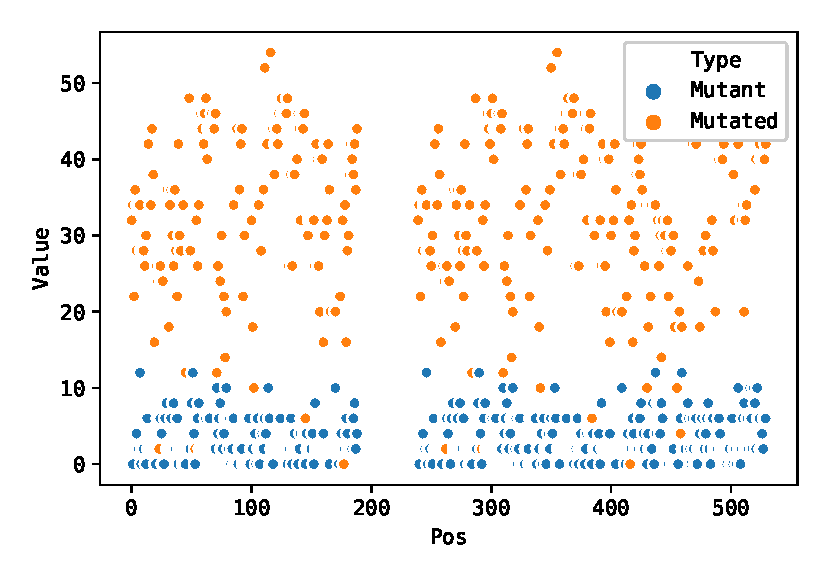
\includegraphics[width=\linewidth]{empirical_evidence_figures/mutate_auction.eps}
%    \caption{Difference in task price to a truthful task and misreported task}
%    \label{fig:auction_mutation}
%\end{figure}
%As the decentralised iterative auction presented in section \ref{subsec:decentralised-iterative-auction} is not
%incentive compatible, it is possible that misreporting of task attribute can decrease the price paid by a task.
%Figure \ref{fig:auction_mutation} is a scatter graph of the  a task (in orange) and the price of a misreported task
%(in blue). Misreported task were generated by increase the task resource requirements or by decreasing the task value
%or deadline that would substituted for the original truthful task. As the figure clearly shows, in almost all cases of
%mutation causes the


\section{Conclusions}\label{sec:conclusions-and-future-work}
In this paper, we studied a resource allocation problem in edge clouds, where resources are elastic and can be
allocated to tasks at varying speeds to satisfy heterogeneous requirements and deadlines. To solve the problem,
we proposed a centralized greedy mechanism with a guaranteed performance bound, and a number of auction-based
mechanisms that also consider the elasticity of resources and limit the potential for strategic manipulation. We show
that explicitly taking advantage of resource elasticity leads to significantly better performance than current
approaches that assume fixed resources.

In future work, we plan to consider the dynamic scenario where tasks arrive and depart from the system over time, and
to also consider the case where task preemption is allowed.
\section{Conclusions and Future work}\label{sec:conclusion-and-future-work}
In this work, we have investigated the possibility of using resource-elastic tasks in edge cloud computing. This ability improves social welfare by 20\% compared to prior work, allowing an expanded use of edge cloud computing when resources are highly limited compared to traditional cloud computing. To do this, we proposed three mechanisms; a greedy approximation algorithm, a centralised incentive compatible auction and a novel decentralised iterative auction. For each algorithm we presented extensive analyses that compare results to the optimal solutions. We also investigated the heuristics of the decentralised iterative auction, the ability to misreport task attributes and the impact of server resource capacity on resource allocation. We have modelled the optimisation problem as a static one-shot case where all of the tasks arrive at the first time step. As part of our future work, we plan to consider a fully online elastic resource allocation optimisation problem. 

\balance

\bibliographystyle{ACM-Reference-Format} 
\bibliography{sections/references}

\end{document}

%%%%%%%%%%%%%%%%%%%%%%%%%%%%%%%%%%%%%%%%%%%%%%%%%%%%%%%%%%%%%%%%%%%%%%%%


